\documentclass[11pt,a4paper]{article}

\usepackage[utf8]{inputenc}
\usepackage[T1]{fontenc}
\usepackage[french]{babel}
\usepackage{amsmath,amssymb}
\usepackage{graphicx}
\usepackage[a4paper,margin=2.5cm]{geometry}
\usepackage{hyperref}
\hypersetup{colorlinks=true,linkcolor=black,urlcolor=blue,citecolor=black}

% Mise en page un peu plus aeree : interligne et espacement entre paragraphes.
\linespread{1.05}
\setlength{\parskip}{0.6em}

\graphicspath{{figures_local/}}

\title{Projet Méthodes Stochastiques\\[0.3em]
       \large Recherche d'un modèle pour le virus $X_t$}
\author{Philippe \textsc{Lin} \and Sayna \textsc{Ren} \and Xuhong \textsc{Liu}}
\date{}

\begin{document}

\maketitle

\textit{Cette note prolonge le rapport principal. Tous les résultats sont reproductibles dans le notebook de recherche qui l'accompagne, où l'on trouve l'ensemble des codes et des figures.}

\section*{Recherche d'un modèle pour le virus $X_t$}

Le premier rapport a reconstruit le virus $X_t$ à partir des données puis mis à l'épreuve le brownien avec dérive et l'Ornstein-Uhlenbeck par un test de Kolmogorov-Smirnov sur les niveaux, sans retenir ni l'un ni l'autre. Plutôt que d'empiler de nouveaux modèles, nous avons eu l'idée de regarder de plus près ce que ce test mesure réellement, ce qui nous a menés à une piste plausible.

\subsection*{Deux signatures du virus reconstruit}

Le virus reconstruit part de $\approx 0$, descend en forme de S vers un plateau autour de $-0{,}58$, et fluctue ensuite faiblement (écart-type du plateau $\approx 0{,}055$). Ses différences $\Delta X_i = X_{i+1}-X_i$ portent deux signatures nettes. Elles sont d'abord symétriques mais à queues lourdes, avec un excès de kurtosis $\approx 3{,}3$ très loin d'une gaussienne. Elles sont ensuite corrélées d'un pas à l'autre, avec une autocorrélation de rang $1$ de l'ordre de $0{,}26$, alors que les modèles à bruit blanc les voudraient indépendantes.

\subsection*{Le test sur les niveaux ne discrimine pas}

Avant de conclure quoi que ce soit d'une p-value faible, nous avons vérifié ce que vaut le test sur les niveaux en comparant une trajectoire de l'Ornstein-Uhlenbeck à une autre trajectoire du \emph{même} modèle. La p-value moyenne reste de l'ordre de $10^{-6}$. Sur des trajectoires aussi longues et aussi corrélées, le test sur les niveaux écarterait donc même le bon modèle, si bien qu'une p-value faible n'y désigne pas un mauvais candidat. Ce qu'un modèle pour $X_t$ fixe réellement, c'est la loi de ses incréments, que nous testons à partir d'ici.

\subsection*{Aucune loi simple ne décrit les incréments natifs}

Au pas natif, des incréments gaussiens donnent une p-value moyenne de l'ordre de $10^{-7}$, écartés par les queues lourdes. Des lois symétriques plus lourdes calées sur la kurtosis, comme la loi de Laplace ou un mélange normal-Gamma, remontent seulement à $10^{-3}$, donc encore largement sous $0{,}05$.

\textbf{À priori, aucune loi simple ne décrit à elle seule les incréments natifs.}

L'échec n'est pas qu'une affaire de queues, puisque les incréments sont aussi corrélés, ce qui trahit une structure de haute fréquence qu'aucune loi i.i.d. ne peut reproduire.

\subsection*{Les queues lourdes sont une structure de haute fréquence}

Si cette structure fine est du bruit de haute fréquence, alors agréger les incréments sur un pas plus grand devrait les rapprocher d'une gaussienne, puisqu'une somme de petits incréments tend vers une loi normale, tout en les décorrélant. Nous avons donc sous-échantillonné $X$ un point sur $k$ et regardé l'évolution de la kurtosis et du test. La figure~\ref{fig:coarse} montre l'excès de kurtosis qui s'effondre vers $0$ tandis que la p-value moyenne d'incréments gaussiens franchit $0{,}05$ dès $dt_k \approx 0{,}03$.

\begin{figure}[ht]
  \centering
  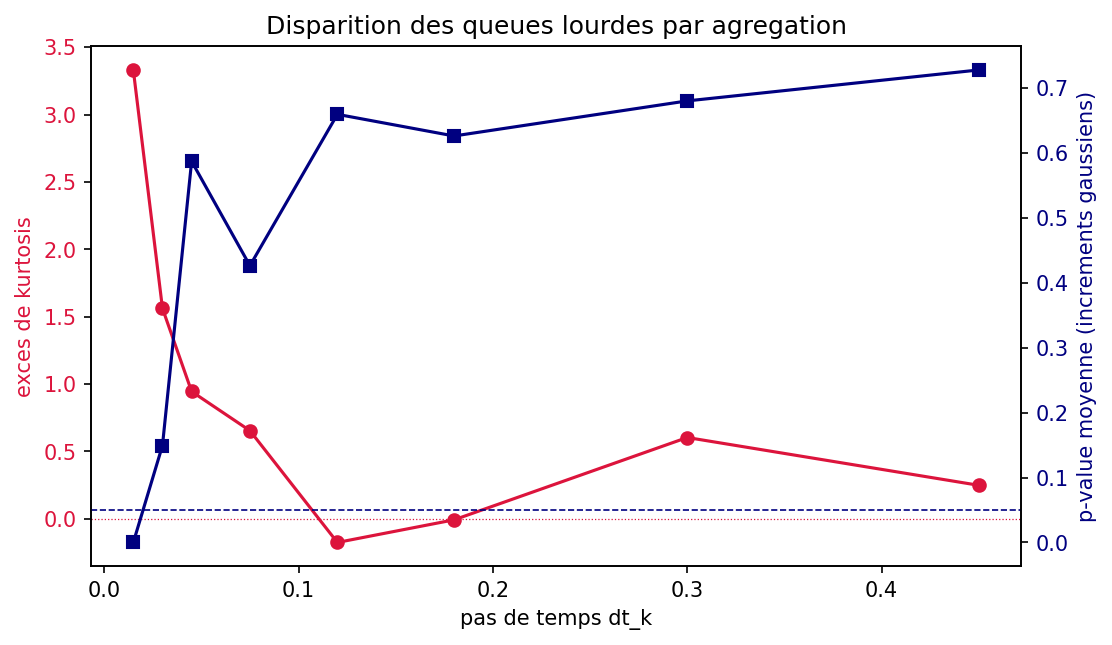
\includegraphics[width=0.8\textwidth]{recherche_coarsegrain.png}
  \caption{Par agrégation des incréments (pas $dt_k = k\,dt$), l'excès de kurtosis (rouge) tombe vers $0$ et la p-value moyenne d'incréments gaussiens (bleu) passe au-dessus de $0{,}05$ (tirets).}
  \label{fig:coarse}
\end{figure}

Au pas $dt_k \approx 0{,}045$ (un point sur trois), l'excès de kurtosis vaut $\approx 0{,}9$, l'autocorrélation est $\approx 0$ et la normalité des incréments n'est plus écartée (p-value $\approx 0{,}84$). La figure~\ref{fig:incr} compare les incréments à une gaussienne, au pas natif puis au pas grossier.

\begin{figure}[ht]
  \centering
  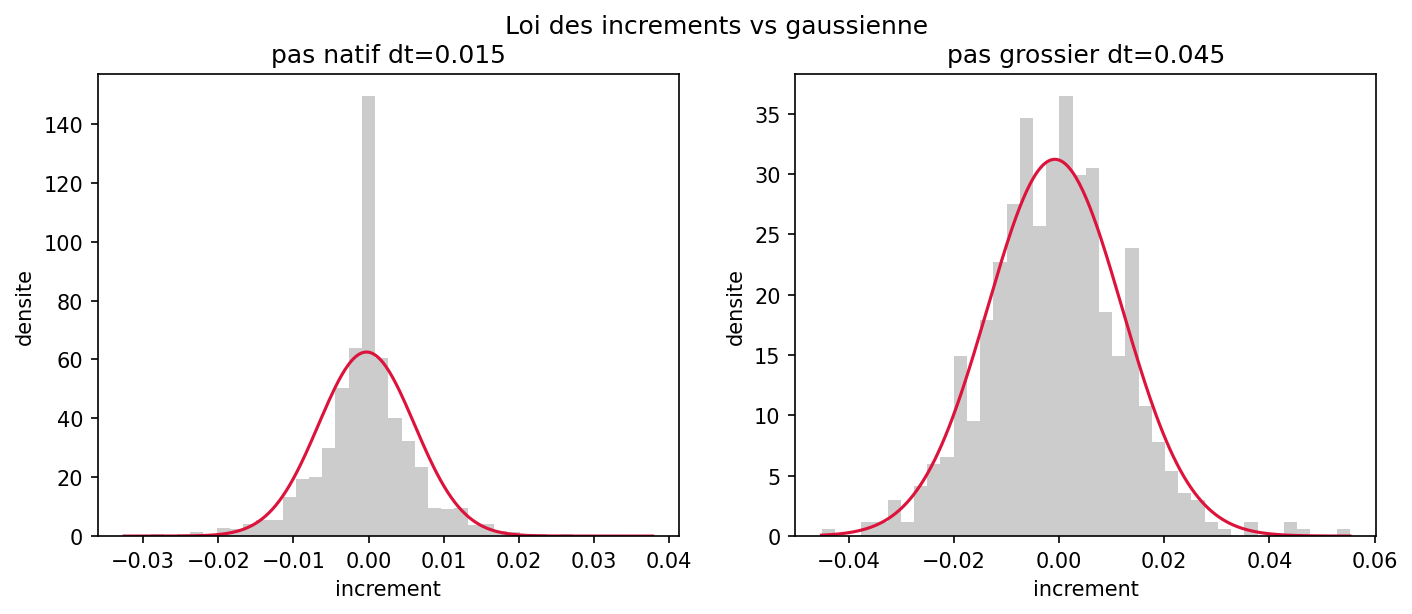
\includegraphics[width=\textwidth]{recherche_increments.png}
  \caption{Loi des incréments comparée à une gaussienne de mêmes moyenne et écart-type, au pas natif (gauche, pic marqué et queues lourdes) et au pas grossier (droite, accord net).}
  \label{fig:incr}
\end{figure}

\subsection*{Test de l'Ornstein-Uhlenbeck au pas grossier}

Au pas grossier, les incréments étant redevenus gaussiens et décorrélés, on retrouve le cadre d'un modèle à bruit blanc. Le plateau traduisant un retour à la moyenne, nous reprenons l'Ornstein-Uhlenbeck. En régressant $\Delta X_i$ sur $X_i$ à ce pas, on trouve :

\begin{center}
  $\theta \approx 0{,}08, \qquad \mu \approx -0{,}63, \qquad \sigma \approx 0{,}06.$
\end{center}

On simule alors $X_t$ par sa solution exacte établie dans le premier rapport, le brownien étant échantillonné au pas grossier (figure~\ref{fig:simou}).

\begin{figure}[ht]
  \centering
  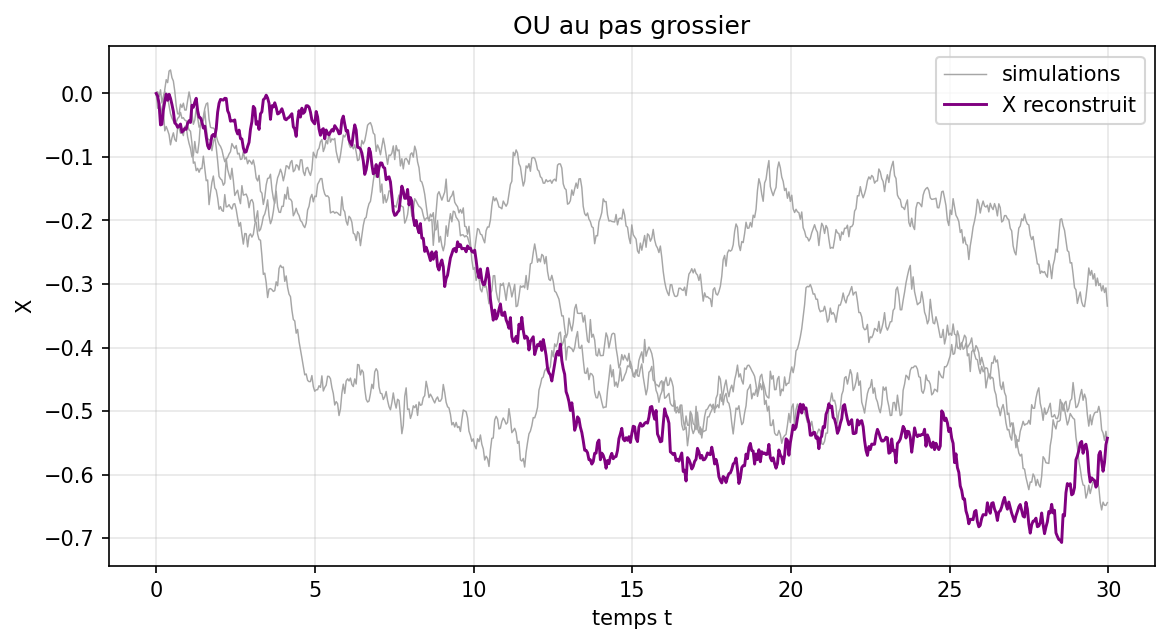
\includegraphics[width=0.6\textwidth]{recherche_sim_ou.png}
  \caption{Trois trajectoires de l'Ornstein-Uhlenbeck au pas grossier (en gris) et le virus reconstruit.}
  \label{fig:simou}
\end{figure}

Le test de Kolmogorov-Smirnov sur les incréments au pas grossier donne une p-value moyenne $\approx 0{,}70$ pour l'Ornstein-Uhlenbeck et $\approx 0{,}60$ pour de simples incréments gaussiens, toutes deux bien au-dessus de $0{,}05$.

\textbf{À priori, l'Ornstein-Uhlenbeck observé au pas grossier reste plausible.}

\subsection*{Bilan}

L'Ornstein-Uhlenbeck observé à un pas un peu plus grand est la piste plausible que nous avons trouvée, la structure fine des incréments ressemblant à du bruit de haute fréquence, très probablement introduit par la dérivation discrète de $V$ lors de la reconstruction. La piste reste imparfaite, puisque l'écart-type stationnaire associé $\sigma/\sqrt{2\theta} \approx 0{,}15$ dépasse le plateau observé $\approx 0{,}055$, et que la descente exponentielle du modèle n'épouse que grossièrement la forme en S des données. La suite naturelle serait un modèle dont la tendance épouse cette forme en S, par exemple une croissance logistique de l'effet du virus.

\end{document}
